\documentclass{article}
\usepackage[T1]{fontenc}
\usepackage[utf8]{inputenc}
\usepackage{lmodern}
\usepackage{amsmath}
\usepackage{sansmath}
\AtBeginDocument{\sansmath}
\renewcommand{\familydefault}{\sfdefault}
\usepackage[paperwidth=19cm,paperheight=14cm,margin=0.4cm]{geometry}
\usepackage{graphicx}
\usepackage{tikz}
\usetikzlibrary{positioning,fit,calc,arrows.meta,backgrounds,decorations.pathreplacing}
\pagestyle{empty}
\setlength{\parindent}{0pt}
\graphicspath{{img/}}

\definecolor{ink}{HTML}{0A0A0A}
\definecolor{muted}{HTML}{6A6A69}
\definecolor{line}{HTML}{BDBDBA}
\definecolor{red}{HTML}{E03A3A}
\definecolor{blue}{HTML}{2E6FE0}
\definecolor{yellow}{HTML}{D9A11A}
\definecolor{green}{HTML}{23A06A}
\definecolor{model}{HTML}{8C8C8A}

\tikzset{
  every picture/.style={font=\sffamily\small, line cap=round, line join=round},
  flecha/.style={-{Stealth[length=2.3mm,width=1.7mm]}, line width=0.7pt, draw=ink},
  grupo/.style={draw=#1, dash pattern=on 3pt off 2pt, line width=0.8pt, rounded corners=2pt, inner sep=6pt},
  titulo/.style={font=\sffamily\small\bfseries, text=#1, anchor=south west, inner sep=1pt},
  foto/.style={inner sep=0pt, outer sep=0pt, draw=ink, line width=0.5pt},
  caja/.style={draw=ink, line width=0.5pt, fill=#1, text=white, font=\sffamily\scriptsize\bfseries,
    text width=3.75cm, minimum height=0.46cm, align=center, inner sep=1.5pt},
  nota/.style={font=\sffamily\scriptsize, text=muted, align=center, inner sep=1pt},
  etapa/.style={font=\sffamily\footnotesize\bfseries, text=ink, align=center, inner sep=1pt},
  paso/.style={draw=ink, line width=0.5pt, fill=#1, text=ink, font=\sffamily\scriptsize, align=center,
    inner sep=3pt, minimum height=0.95cm, text width=2.35cm},
  paso/.default=white,
  grupofondo/.style={draw=#1, line width=0.8pt, fill=#1!6, rounded corners=3pt, inner sep=7pt},
  llave/.style={decorate, decoration={brace, mirror, amplitude=5pt, raise=2pt}, line width=0.7pt, draw=#1},
  llavetexto/.style={font=\sffamily\small\bfseries, text=#1, align=center},
}

\begin{document}
\begin{tikzpicture}

\node[foto] (s1) at (0, 0) {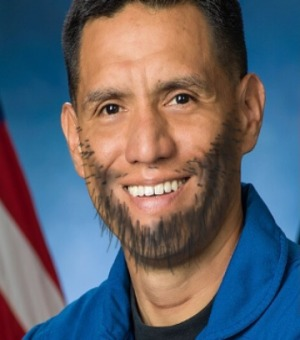
\includegraphics[width=1.8cm]{f_reposo.jpg}};
\node[etapa, above=4pt of s1] {Cámara};
\node[nota, below=3pt of s1] (n1) {unos 10 cuadros\\por segundo};

\node[paso, text width=2.2cm, minimum height=1.8cm] (s2) at (2.55, 0) {%
  \textbf{Seguimiento}\\[2pt]MediaPipe en video\\y filtro One-Euro\\contra el temblor};

\node[paso, text width=2.2cm, minimum height=1.8cm] (s3) at (5.15, 0) {%
  \textbf{Anclaje}\\[2pt]cada raíz guarda\\sus coordenadas\\baricéntricas};

\begin{scope}[shift={(7.75, 0.75)}]
  \draw[ink, line width=1.6pt] (-0.75, 0) -- (0.75, 0);
  \node[nota, anchor=south] at (0, 0.04) {piel};
  \draw[muted, line width=0.6pt, dash pattern=on 2pt off 1.5pt] (0, 0) -- (0, -1.5);
  \coordinate (p0) at (0, 0);
  \coordinate (p1) at (-0.1, -0.5);
  \coordinate (p2) at (-0.32, -0.97);
  \coordinate (p3) at (-0.62, -1.38);
  \draw[red, line width=1pt] (p0) -- (p1) -- (p2) -- (p3);
  \foreach \p in {p0, p1, p2, p3} { \fill[ink] (\p) circle (0.065); }
  \draw[flecha, line width=0.5pt] (0.45, -0.55) -- (0.45, -1.05) node[midway, right=1pt, nota] {$g$};
  \node[nota, anchor=north west, align=left] at (0.15, -1.15) {reposo};
\end{scope}
\node[etapa, anchor=south] at ($(7.75, 0 |- s1.north) + (0, 0.1)$) {Física};
\node[nota] (n4) at (7.75, 0 |- n1) {Verlet amortiguado y\\restricción de largo (PBD)};

\node[paso, text width=2.2cm, minimum height=1.8cm] (s5) at (10.35, 0) {%
  \textbf{Render}\\[2pt]cada tramo es una\\gaussiana 2D;\\$\alpha = 1 - e^{-A}$};

\node[foto] (s6) at (12.9, 0) {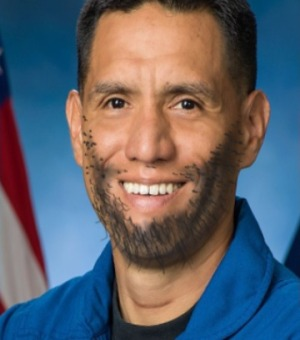
\includegraphics[width=1.8cm]{f_movimiento.jpg}};
\node[etapa, above=4pt of s6] {Resultado};
\node[nota, below=3pt of s6] (n6) {las puntas se\\atrasan y vuelven};

\draw[flecha] (s1) -- (s2);
\draw[flecha] (s2) -- (s3);
\draw[flecha] (s3) -- (6.85, 0);
\draw[flecha] (8.65, 0) -- (s5);
\draw[flecha] (s5) -- (s6);

\coordinate (base) at ($(n4.south) + (0, -0.06)$);
\draw[llave=muted] (s2.west |- base) -- (s2.east |- base)
  node[midway, below=9pt, llavetexto=muted] {Modelo};
\draw[llave=ink] (s3.west |- base) -- (s5.east |- base)
  node[midway, below=9pt, llavetexto=ink] {Implementado por el equipo};

\end{tikzpicture}
\end{document}
